%%%%%%%%%%%%%%%%%%%%%%%%%%%%%%%%%%%%%%%%%
% Beamer Presentation
% LaTeX Template
%
% This template has been downloaded from:
% http://www.LaTeXTemplates.com
%
% This template has been altered after it was downloaded from the 
% above link
%
% License:
% CC BY-NC-SA 3.0 (http://creativecommons.org/licenses/by-nc-sa/3.0/)
%
%%%%%%%%%%%%%%%%%%%%%%%%%%%%%%%%%%%%%%%%%

%----------------------------------------------------------------------------------------
%	PACKAGES AND THEMES


\documentclass{beamer}

\mode<presentation> {

% The Beamer class comes with a number of default slide themes
% which change the colors and layouts of slides. Below this is a list
% of all the themes, uncomment each in turn to see what they look like.

%\usetheme{default}
%\usetheme{AnnArbor}
%\usetheme{Antibes}
%\usetheme{Bergen}
%\usetheme{Berkeley}
%\usetheme{Berlin}
\usetheme{Boadilla}
%\usetheme{CambridgeUS}
%\usetheme{Copenhagen}
%\usetheme{Darmstadt}
%\usetheme{Dresden}
%\usetheme{Frankfurt}
%\usetheme{Goettingen}
%\usetheme{Hannover}
%\usetheme{Ilmenau}
%\usetheme{JuanLesPins}
%\usetheme{Luebeck}
%\usetheme{Madrid}
%\usetheme{Malmoe}
%\usetheme{Marburg}
%\usetheme{Montpellier}
%\usetheme{PaloAlto}
%\usetheme{Pittsburgh}
%\usetheme{Rochester}
%\usetheme{Singapore}
%\usetheme{Szeged}
%\usetheme{Warsaw}

% As well as themes, the Beamer class has a number of color themes
% for any slide theme. Uncomment each of these in turn to see how it
% changes the colors of your current slide theme.

%\usecolortheme{albatross}
%\usecolortheme{beaver}
%\usecolortheme{beetle}
%\usecolortheme{crane}
%\usecolortheme{dolphin}
%\usecolortheme{dove}
%\usecolortheme{fly}
%\usecolortheme{lily}
%\usecolortheme{orchid}
%\usecolortheme{rose}
\usecolortheme{seagull}
%\usecolortheme{seahorse}
%\usecolortheme{whale}
%\usecolortheme{wolverine}

% Here is an overview of possible theme and colortheme combinations:
% https://hartwork.org/beamer-theme-matrix/

%\setbeamertemplate{footline} % To remove the footer line in all slides uncomment this line
%\setbeamertemplate{footline}[page number] % To replace the footer line in all slides with a simple slide count uncomment this line

\setbeamertemplate{navigation symbols}{} % To remove the navigation symbols from the bottom of all slides uncomment this line
}

\usepackage[english]{babel}
\usepackage[autostyle, english = american]{csquotes}
\MakeOuterQuote{"}

\usepackage{graphicx} % Allows including images
\usepackage{booktabs} % Allows the use of \toprule, \midrule and \bottomrule in tables
\usepackage{appendixnumberbeamer} % Allows use of \appendix. Slides appearing after will not be part of the frame counter or navigation panel
\usepackage{todonotes} % Allows use of \missingfigure

\usepackage{mathtools}
\usepackage{hyperref}
\hypersetup{
	colorlinks=true,
	linkcolor=black,      
	urlcolor=blue
}

\usepackage[all]{xy}

\newcommand\blfootnote[1]{%
	\begingroup
	\renewcommand\thefootnote{}\footnote{#1}%
	\addtocounter{footnote}{-1}%
	\endgroup
}

\newcommand{\btheta}{\boldsymbol{\theta}} 
\newcommand{\bphi}{\boldsymbol{\phi}}

% Following lines makes a section overview at the beginning of each section 
\setbeamertemplate{caption}{\raggedright\insertcaption\par}
\AtBeginSection[]
{
 \begin{frame}<beamer>
 %\frametitle{Plan}
 \tableofcontents[currentsection]
 \end{frame}
}

%----------------------------------------------------------------------------------------
%   TITLE PAGE
%----------------------------------------------------------------------------------------

\title[Week 10]{Generative Modeling for EEG Classification via Signal Filtering} % The short title appears at the bottom of every slide (dependent on theme), the full title is only on the title page

\author{Artyom Matveev} % Your name
\institute[MIPT] % Your institution as it will appear on every slide (dependent on theme), may be shorthand to save space
{
Moscow Institute of Physics and Technology \\ % Your institution for the title page
\medskip
\textit{matveev.as@phystech.edu} % Your email address
}
\date{November 25, 2023} % Date, can be changed to a custom date

\begin{document}

{
%\usebackgroundtemplate{\includegraphics[width=\paperwidth]{figures/background.jpg}} % background of first slide
\begin{frame}
\titlepage % Print the title page as the first slide
\end{frame}
}

%\begin{frame}
%\frametitle{Overview} % Table of contents slide, comment this block out to remove it
%\tableofcontents % Throughout your presentation, if you choose to use \section{} and \subsection{} commands, these will automatically be printed on this slide as an overview of your presentation
%\end{frame}

%----------------------------------------------------------------------------------------
%   PRESENTATION SLIDES
%----------------------------------------------------------------------------------------

%------------------------------------------------
%\section{First Section} % Sections can be created in order to organize your presentation into discrete blocks, all sections and subsections are automatically printed in the table of contents as an overview of the talk
%%------------------------------------------------
%
%\subsection{Subsection Example} % A subsection can be created just before a set of slides with a common theme to further break down your presentation into chunks

\begin{frame}{Project description}
\begin{enumerate}
\item \textbf{Title}: "Generative Modeling for EEG Classification via Signal Filtering"
\item \textbf{Problem}: solve an EEG classification task. 
\item \textbf{Data}: \href{https://neurotechx.github.io/moabb/dataset\_summary.html}{EEG datasets} from MOABB library. 
%\item \textbf{Reference}:  
\item \textbf{Base solution}: Riemannian-based kernel approach by A. Barachant.
\item \textbf{Proposed solution}: solve the task by using a decision-rejection strategy. First, we learn two probabilistic models for known ($p(\mathbf{X} | \btheta)$) and new ($q(\mathbf{Y} | \bphi)$) data. Then, we measure the distance of these distributions and reject patterns from $q(\mathbf{Y} | \bphi)$ that don't belong to expected patterns in $p(\mathbf{X} | \btheta)$.
\item \textbf{Novelty}: the proposed solution is universal, it doesn't depend on specific class of EEG data (Motor Imagery, SSVEP, P300, etc.) because we represent the data as probability distributions. 
%\begin{center}
%	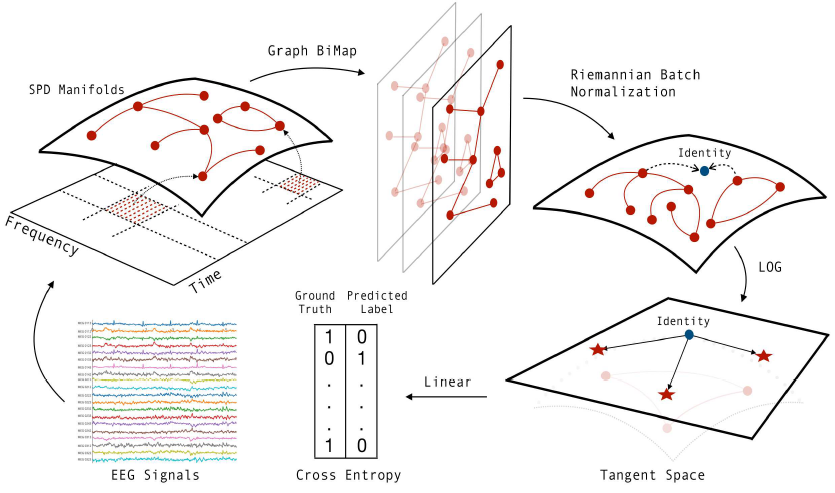
\includegraphics[height = 3.5cm, width=6.5cm]{images/2023_Ju.png}
%\end{center}

%\begin{xy}
%	% Your xy-pic diagram code here
%	\xymatrix{
%		\bullet \ar@/^/[r]
%		\ar@/_/@{.>}[r] &
%		\bullet }
%		
%	(0,20)*{\includegraphics[height=0.1\textheight, width=0.1\textwidth]{./images/pngwing.png}};
%\end{xy}

\end{enumerate}

%\blfootnote{\tiny{\textbf{Barachant, A.}, Bonnet, S., et al. Multiclass brain-computer interface classification by Riemannian geometry. 2012}}
\end{frame}
\end{document} 